\documentclass[12pt,a4paper]{article}

% ==============================================================================
% 1. CÁC GÓI CƠ BẢN VÀ ĐỊNH DẠNG TIẾNG VIỆT
% ==============================================================================
\usepackage[utf8]{vietnam}              % Hỗ trợ gõ tiếng Việt có dấu chuẩn TCVN/Unicode
\usepackage[english,vietnamese]{babel}  % Thiết lập ngôn ngữ
\usepackage{amsmath,amssymb,amsfonts}  % Hỗ trợ công thức toán học
\usepackage{graphicx}                   % Chèn hình ảnh
\usepackage{subcaption}                 % Hỗ trợ môi trường subfigure
\usepackage{booktabs}                   % Bảng chuẩn khoa học (toprule, midrule, bottomrule)
\usepackage{multirow}                   % Gộp dòng trong bảng
\usepackage{array}                      % Tùy biến cột bảng
\usepackage{xcolor}                     % Màu sắc
\usepackage{qrcode}                     % Tự động tạo mã QR Code trong PDF
\usepackage{listings}                   % Chèn mã nguồn code nếu cần
\usepackage{tcolorbox}                  % Khung màu làm nổi bật nội dung

% Định dạng lề trang chuẩn báo cáo khoa học (A4)
\usepackage[top=2.5cm, bottom=2.5cm, left=3.0cm, right=2.0cm]{geometry}

% ==============================================================================
% 2. THƯ VIỆN ĐỒ HỌA TIKZ & PGFPLOTS (BẮT BUỘC THEO YÊU CẦU ĐẶC BIỆT)
% ==============================================================================
\usepackage{tikz}
\usepackage{pgfplots}
\pgfplotsset{compat=1.18}
\usetikzlibrary{
    shapes.geometric, 
    shapes.misc,
    arrows.meta, 
    positioning, 
    calc, 
    shadows.blur,
    fit,
    backgrounds
}

% Định nghĩa màu sắc nhận diện thương hiệu IoT & Smart Classroom
\definecolor{iotBlue}{HTML}{1A73E8}
\definecolor{iotGreen}{HTML}{28A745}
\definecolor{iotRed}{HTML}{DC3545}
\definecolor{iotCyan}{HTML}{00A8CC}
\definecolor{iotAmber}{HTML}{F59E0B}
\definecolor{iotDark}{HTML}{0F172A}
\definecolor{boxBgBlue}{HTML}{EBF3FD}
\definecolor{boxBgGreen}{HTML}{EAF7ED}
\definecolor{boxBgRed}{HTML}{FDE8EA}
\definecolor{boxBgCyan}{HTML}{E6F7FA}
\definecolor{boxBgPurple}{HTML}{F3E8FD}

% Cấu hình liên kết Hyperref
\usepackage{hyperref}
\hypersetup{
    colorlinks=true,
    linkcolor=iotBlue,
    filecolor=magenta,      
    urlcolor=iotBlue,
    citecolor=iotGreen,
    pdftitle={SMART CLASSROOM IoT SYSTEM - Báo Cáo Kỹ Thuật},
    pdfauthor={Nhóm Nghiên Cứu IOT102},
    pdfsubject={Hệ thống Giám sát và Tự động hóa Phòng học Thông minh},
    pdfkeywords={ESP8266, IoT, Smart Classroom, DHT11, MQ135, PIR, Non-blocking}
}

% Cấu hình Header và Footer
\usepackage{fancyhdr}
\pagestyle{fancy}
\fancyhf{}
\fancyhead[L]{\small\color{gray} Đồ án Capstone IOT102: \textbf{Smart Classroom IoT System}}
\fancyhead[R]{\small\color{gray} Vi điều khiển ESP8266}
\fancyfoot[L]{\small\color{gray} Bộ môn Kỹ thuật Máy tính / IoT}
\fancyfoot[R]{\thepage}
\renewcommand{\headrulewidth}{0.4pt}
\renewcommand{\footrulewidth}{0.4pt}

% ==============================================================================
% THIẾT KẾ CÁC STYLE TIKZ CHUẨN KỸ THUẬT CHO BLOCK DIAGRAM & FLOWCHART
% ==============================================================================
\tikzset{
    % --- STYLES CHO BLOCK DIAGRAM (S8) ---
    block_input/.style={
        rectangle, 
        rounded corners=8pt, 
        minimum width=3.4cm, 
        minimum height=1.15cm, 
        text centered, 
        draw=iotBlue!80!black, 
        fill=boxBgBlue, 
        line width=1.2pt, 
        font=\small\bfseries,
        blur shadow={shadow blur steps=3, shadow xshift=1pt, shadow yshift=-1pt, shadow opacity=20}
    },
    block_output/.style={
        rectangle, 
        rounded corners=8pt, 
        minimum width=3.4cm, 
        minimum height=1.05cm, 
        text centered, 
        draw=iotGreen!80!black, 
        fill=boxBgGreen, 
        line width=1.2pt, 
        font=\small\bfseries,
        blur shadow={shadow blur steps=3, shadow xshift=1pt, shadow yshift=-1pt, shadow opacity=20}
    },
    block_server/.style={
        rectangle, 
        rounded corners=8pt, 
        minimum width=4.5cm, 
        minimum height=1.3cm, 
        text centered, 
        draw=purple!80!black, 
        fill=boxBgPurple, 
        line width=1.2pt, 
        font=\small\bfseries,
        blur shadow={shadow blur steps=3, shadow xshift=1pt, shadow yshift=-1pt, shadow opacity=20}
    },
    block_controller/.style={
        rectangle, 
        rounded corners=12pt, 
        minimum width=5.8cm, 
        minimum height=7.2cm, 
        text centered, 
        draw=iotCyan!90!black, 
        fill=boxBgCyan, 
        line width=1.8pt,
        blur shadow={shadow blur steps=5, shadow xshift=2pt, shadow yshift=-2pt, shadow opacity=25}
    },
    sub_module/.style={
        rectangle, 
        rounded corners=5pt, 
        minimum width=5.0cm, 
        minimum height=0.95cm, 
        text centered, 
        draw=iotCyan!70!black, 
        fill=white, 
        line width=0.9pt, 
        font=\footnotesize
    },
    sig_arrow/.style={
        -{Stealth[length=2.8mm,width=2.2mm]}, 
        line width=1.2pt, 
        draw=iotDark!80
    },
    sig_bi/.style={
        {Stealth[length=2.8mm,width=2.2mm]}-{Stealth[length=2.8mm,width=2.2mm]}, 
        line width=1.3pt, 
        draw=purple!80!black
    },
    % --- STYLES CHO FLOWCHART (S9) ---
    fc_start/.style={
        rounded rectangle, 
        minimum width=3.6cm, 
        minimum height=0.9cm, 
        text centered, 
        draw=iotBlue!90!black, 
        fill=boxBgBlue, 
        line width=1.2pt, 
        font=\small\bfseries
    },
    fc_proc/.style={
        rectangle, 
        rounded corners=4pt, 
        minimum width=4.5cm, 
        minimum height=0.95cm, 
        text centered, 
        draw=slate!80!black, 
        fill=gray!10, 
        line width=1.0pt, 
        font=\footnotesize
    },
    fc_dec/.style={
        diamond, 
        aspect=2.4, 
        text centered, 
        draw=iotAmber!90!black, 
        fill=iotAmber!15, 
        line width=1.1pt, 
        font=\footnotesize\bfseries
    },
    fc_arrow/.style={
        -{Stealth[length=2.5mm,width=2.0mm]}, 
        line width=1.1pt, 
        draw=iotDark!85
    }
}

% ==============================================================================
% BẮT ĐẦU NỘI DUNG TÀI LIỆU
% ==============================================================================
\begin{document}

% ------------------------------------------------------------------------------
% S1 & S2: TRANG BÌA & THÔNG TIN THÀNH VIÊN ĐỀ TÀI
% ------------------------------------------------------------------------------
\begin{titlepage}
    \centering
    \vspace*{0.5cm}
    
    {\fontsize{15}{18}\selectfont \textbf{TRƯỜNG ĐẠI HỌC FPT}}\\[0.2cm]
    {\fontsize{13}{16}\selectfont \textbf{BỘ MÔN KỸ THUẬT ĐIỀU KHIỂN \& INTERNET OF THINGS}}\\[1.5cm]

    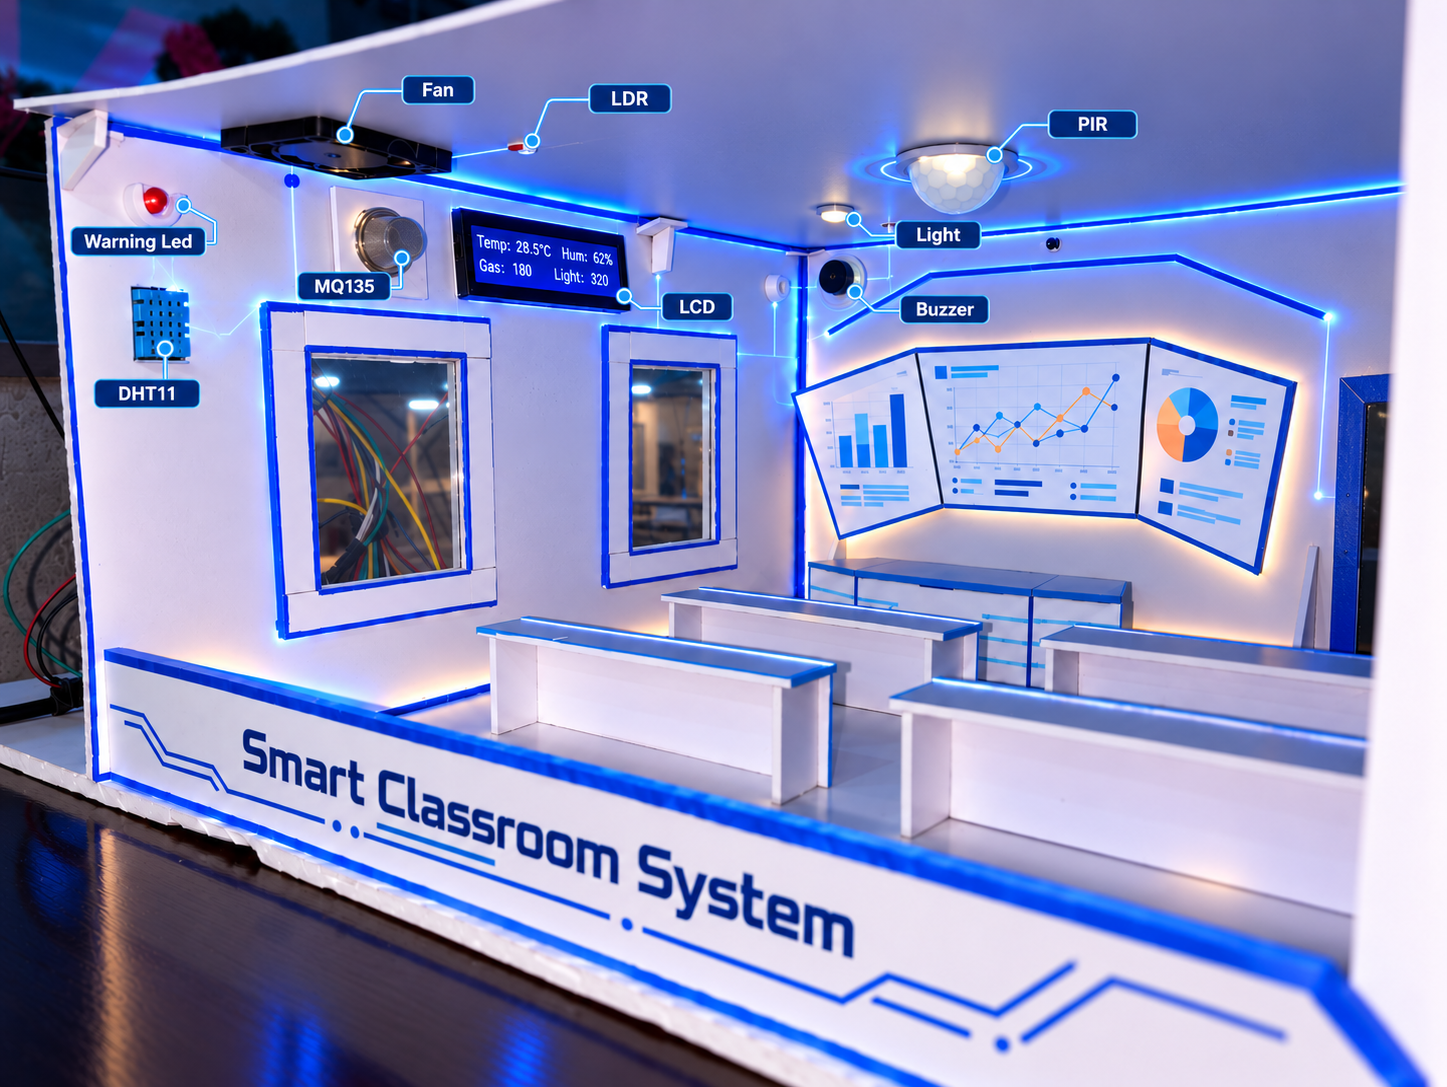
\includegraphics[width=4.5cm]{Smart Classroom System Diorama.png}\\[1.5cm]

    {\color{iotBlue}\rule{\linewidth}{1.6pt}}\\[0.4cm]
    {\fontsize{20}{24}\selectfont \textbf{BÁO CÁO KỸ THUẬT ĐỒ ÁN CAPSTONE}}\\[0.3cm]
    {\fontsize{17}{22}\selectfont \textbf{SMART CLASSROOM IoT SYSTEM}}\\[0.2cm]
    {\fontsize{13}{16}\selectfont \textit{Hệ thống Giám sát An toàn và Tự động hóa Phòng học Thông minh\\dựa trên Vi điều khiển ESP8266}}\\[0.2cm]
    {\color{iotBlue}\rule{\linewidth}{1.6pt}}\\[1.5cm]

    \begin{minipage}{0.9\textwidth}
        \textbf{Thông tin nhóm nghiên cứu đề tài:}
        \begin{table}[h!]
            \centering
            \begin{tabular}{@{}llll@{}}
                \toprule
                \textbf{STT} & \textbf{Họ và Tên} & \textbf{MSSV} & \textbf{Vai Trò Chuyên Trách} \\
                \midrule
                1 & Nguyễn Văn A & SE170001 & Firmware Lead (ESP8266 Non-blocking Core) \\
                2 & Trần Thị B   & SE170002 & Hardware Engineer (Mạch Fritzing \& Sensors) \\
                3 & Lê Văn C     & SE170003 & Cloud/Web Dev (Dashboard \& Google Webhook) \\
                4 & Phạm Văn D   & SE170004 & QA \& Documentation (Kiểm thử 4 Test Cases) \\
                \bottomrule
            \end{tabular}
        \end{table}
    \end{minipage}

    \vfill
    {\large \textbf{Học kỳ: Fall 2026 -- Khóa học IOT102}}\\[0.2cm]
    {\small Hà Nội, Tháng 11 Năm 2026}
\end{titlepage}

\newpage
% ------------------------------------------------------------------------------
% S5: MỤC LỤC TỰ ĐỘNG
% ------------------------------------------------------------------------------
\tableofcontents
\vspace{0.8cm}
\listoffigures
\vspace{0.8cm}
\listoftables
\newpage

% ------------------------------------------------------------------------------
% S3 & S4: BỐI CẢNH & GIỚI THIỆU TỔNG QUAN GIẢI PHÁP
% ------------------------------------------------------------------------------
\section{Bối Cảnh, Tính Cấp Thiết \& Giới Thiệu Sản Phẩm}

\subsection{Bối Cảnh Khách Quan và Các Vấn Đề Tồn Tại (S3)}
Trong các cơ sở giáo dục đại học và phổ thông hiện nay, công tác quản lý năng lượng và an toàn trường học đang đối mặt với ba thách thức nghiêm trọng:
\begin{enumerate}
    \item \textbf{Lãng phí năng lượng điện quy mô lớn:} Sinh viên và cán bộ giảng dạy thường xuyên quên ngắt hệ thống đèn chiếu sáng và quạt sau khi kết thúc buổi học. Việc thiết bị vận hành không tải suốt đêm và các ngày nghỉ cuối tuần gây thất thoát hàng trăm nghìn kWh điện mỗi năm, làm gia tăng chi phí vận hành cho nhà trường.
    \item \textbf{Rủi ro cháy nổ và rò rỉ khí gas ngoài giờ hành chính:} Tại các phòng thí nghiệm Lý -- Hóa hoặc phòng thực hành, các sự cố rò rỉ khí gas, khói phát sinh âm ỉ từ chập điện thường xảy ra ngoài giờ học khi không có người trực. Sự thiếu vắng hệ thống giám sát từ xa dẫn đến nguy cơ bùng phát hỏa hoạn nghiêm trọng.
    \item \textbf{Sự thụ động của hệ thống công tắc cơ truyền thống:} Công tắc cơ hoàn toàn phụ thuộc vào hành vi và ý thức người dùng. Hệ thống không có khả năng tự nhận thức ngữ cảnh môi trường (Context-aware), không lưu vết dữ liệu và không thể điều khiển dự phòng khi xảy ra sự cố.
\end{enumerate}

\subsection{Tổng Quan Giải Pháp Smart Classroom IoT (S4)}
Đồ án xây dựng hệ thống nhúng thông minh hoàn chỉnh dựa trên vi điều khiển ESP8266, kết hợp kiến trúc tính toán tại biên (\textit{Edge Computing}) và dịch vụ phân phối thông điệp đám mây (\textit{Cloud Webhook}):
\begin{itemize}
    \item \textbf{Tự động hóa Đèn/Quạt thích ứng:} Kết hợp điều kiện logic giữa cảm biến chuyển động hồng ngoại PIR (HC-SR501) và cảm biến quang trở (LDR) để chỉ bật đèn khi có người và phòng tối. Điều khiển quạt tản nhiệt tự động dựa trên nhiệt độ đo được từ cảm biến DHT11 với thuật toán trễ (Hysteresis) $0.5^\circ\text{C}$ chống rung giật rơ-le.
    \item \textbf{Giám sát đa cảm biến thời gian thực:} Thu thập song song dữ liệu nhiệt độ, độ ẩm, nồng độ khí độc/gas (MQ135), chuyển động và ánh sáng theo kiến trúc Non-blocking $2000\,\text{ms}$, đồng thời hiển thị thông số trên LCD 1602 qua giao tiếp I2C.
    \item \textbf{Web Server Dashboard nội bộ \& Chế độ dự phòng AP Fallback:} Tích hợp Web Server trên cổng tiêu chuẩn 80. Khi mất kết nối WiFi trường quá 15 giây, thiết bị tự động chuyển sang chế độ Access Point độc lập (\texttt{192.168.4.1}) giúp duy trì kiểm soát liên tục.
    \item \textbf{Cảnh báo khẩn cấp qua Email HTML thông minh:} Kết nối API Google Apps Script Webhook. Áp dụng cơ chế phân loại cảnh báo leo thang (\textit{Escalation Alert}) kết hợp khoảng thời gian nghỉ (\textit{Cooldown}) 5 phút nhằm loại bỏ hoàn toàn hiện tượng bão thư rác (Spam flooding).
\end{itemize}

\newpage
% ------------------------------------------------------------------------------
% S6: HỆ THỐNG CẢM BIẾN, THIẾT BỊ CHẤP HÀNH VÀ BẢNG PHÂN BỔ CHÂN (PINOUT)
% ------------------------------------------------------------------------------
\section{Phân Tích Cảm Biến, Thiết Bị Chấp Hành \& Bảng Pinout (S6)}

Hệ thống sử dụng các linh kiện chuyên dụng, được tối ưu hóa chân cắm trên nền tảng ESP8266 NodeMCU V3 như trình bày trong Bảng~\ref{tab:pinout_mapping}.

\begin{table}[htbp]
    \centering
    \caption{Bảng phân bổ chân cắm (Pinout Mapping) và thông số kỹ thuật của hệ thống}
    \label{tab:pinout_mapping}
    \begin{tabular}{@{}llccp{6.8cm}@{}}
        \toprule
        \textbf{Thiết Bị / Module} & \textbf{Ký Hiệu} & \textbf{Chân ESP} & \textbf{Chuẩn Tín Hiệu} & \textbf{Quy Tắc Điều Khiển \& Ngưỡng Kích Hoạt} \\
        \midrule
        \multicolumn{5}{@{}l}{\textbf{A. Cảm biến đầu vào (Inputs)}} \\
        DHT11 Sensor & D3 & GPIO0 & 1-Wire Digital & Đo nhiệt độ \& độ ẩm. Bật quạt/cảnh báo khi $T \ge 30.0^\circ\text{C}$, ngắt khi $T \le 29.5^\circ\text{C}$ (Hysteresis $0.5^\circ\text{C}$). \\
        MQ135 Gas Sensor & A0 & ADC0 & Analog (10-bit) & Đo nồng độ khí gas/khói độc ($0 - 1023$). Hú còi báo động khi $\text{ADC} \ge 500$, tắt còi khi $\le 450$. \\
        PIR HC-SR501 & D5 & GPIO14 & Hardware ISR & Phát hiện chuyển động bằng ngắt ngoài (\texttt{RISING}). Giữ trạng thái đèn sáng $15\,\text{s}$ (\texttt{PIR\_HOLD\_TIME}). \\
        LDR Quang trở & D6 & GPIO12 & Digital In & Xác định môi trường Tối/Sáng. Điều kiện bật đèn: $\text{Tối} \land \text{Có chuyển động}$. \\
        \midrule
        \multicolumn{5}{@{}l}{\textbf{B. Thiết bị điều khiển đầu ra (Outputs)}} \\
        Relay Quạt & D0 & GPIO16 & Active High & Đóng cắt nguồn cho quạt tản nhiệt làm mát phòng. \\
        LED Đèn Học & D4 & GPIO2 & Active Low & Đèn chiếu sáng học tập tự động tiết kiệm năng lượng. \\
        Warning LED & D7 & GPIO13 & Active High & LED đỏ nhấp nháy chu kỳ $300\,\text{ms}$ khi xảy ra sự cố. \\
        Còi Buzzer & D8 & GPIO15 & Active High & Phát âm thanh cảnh báo mức âm lượng cao khi nồng độ gas nguy hiểm. \\
        LCD 1602 Display & D1/D2 & GPIO5/4 & I2C (Addr \texttt{0x27}) & D1: SCL, D2: SDA. Luân phiên đổi màn hình thông số mỗi $2\,\text{s}$. \\
        \bottomrule
    \end{tabular}
\end{table}

\newpage
% ------------------------------------------------------------------------------
% S7: SƠ ĐỒ ĐẤU NỐI MẠCH FRITZING
% ------------------------------------------------------------------------------
\section{Sơ Đồ Nguyên Lý Đấu Dây Fritzing (S7)}

Sơ đồ đấu nối phần cứng chi tiết của hệ thống Smart Classroom IoT được thiết kế và mô phỏng hoàn chỉnh trên phần mềm Fritzing CAD. Mô hình thực tế sử dụng chung một đường mass (Common Ground) giữa nguồn cấp $5\,\text{V}$ DC và vi điều khiển ESP8266 để triệt tiêu nhiễu tín hiệu.

\begin{figure}[htbp]
    \centering
    % Placeholder chèn ảnh fritzing_wiring.png
    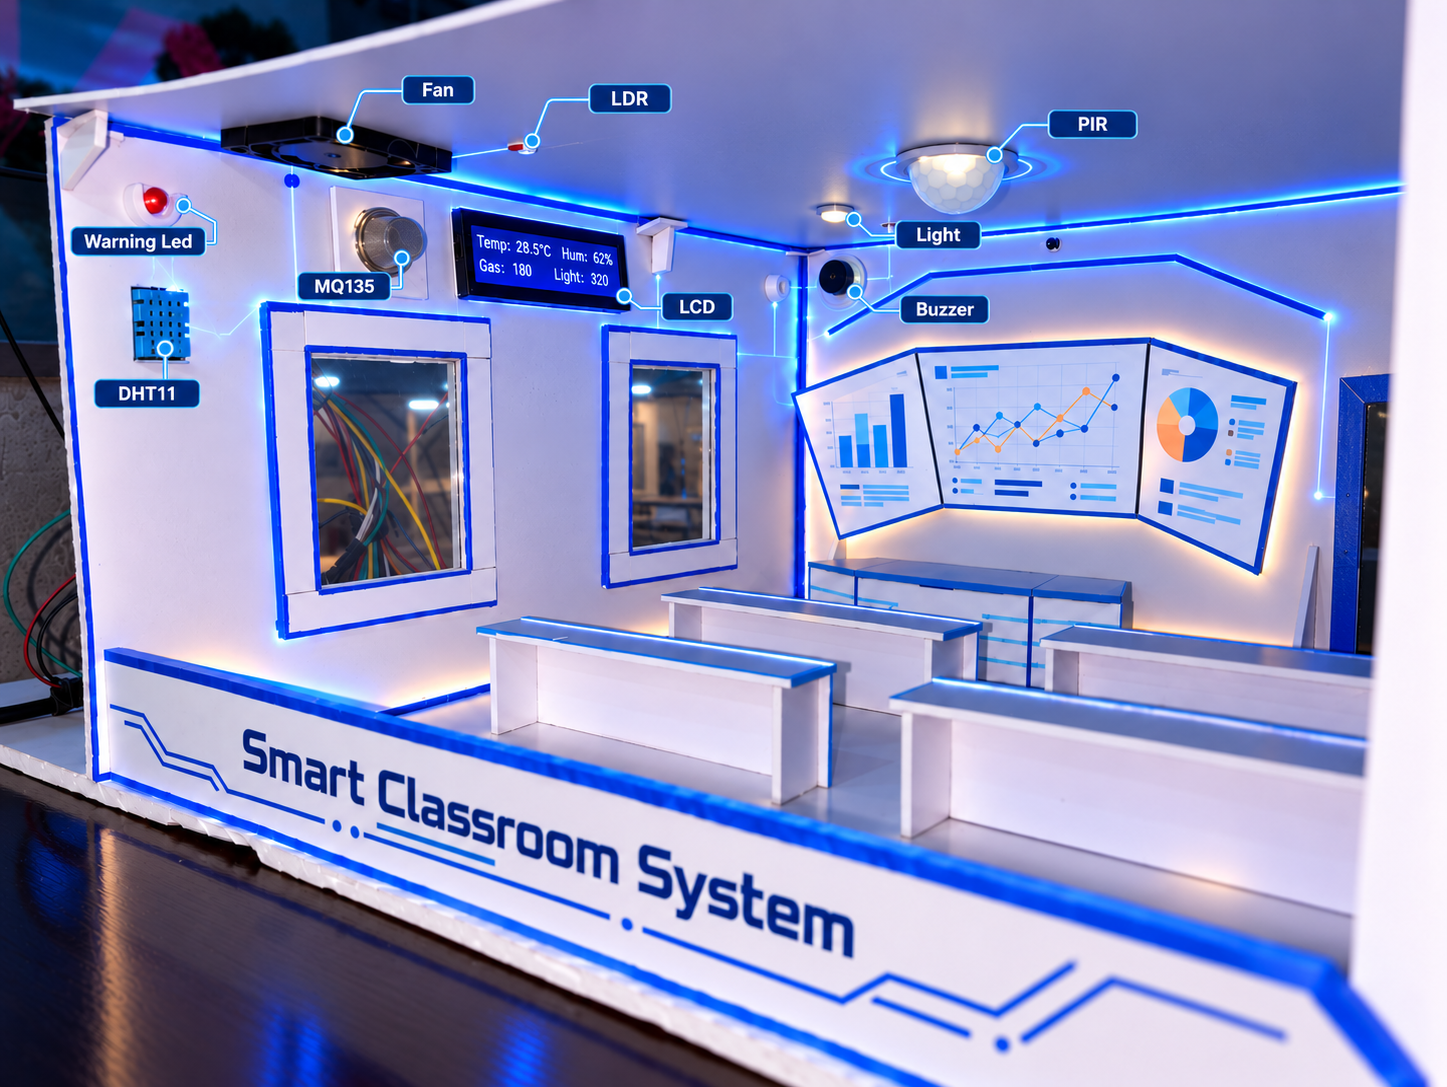
\includegraphics[width=0.88\textwidth, height=9.0cm, keepaspectratio]{Smart Classroom System Diorama.png}
    \caption{Sơ đồ nguyên lý đấu dây Fritzing toàn diện của hệ thống Smart Classroom IoT}
    \label{fig:fritzing_schematic}
\end{figure}

\begin{tcolorbox}[colback=boxBgBlue, colframe=iotBlue, title=\textbf{Nguyên tắc bảo vệ phần cứng khi lắp ráp mạch}]
    \begin{itemize}
        \item \textbf{Bảo vệ chân GPIO15 (D8):} Chân này phải ở mức LOW trong quá trình khởi động ESP8266 (Bootloader). Do đó, mạch gắn Buzzer được kết nối thông qua điện trở kéo xuống (Pull-down $10\,\text{k}\Omega$).
        \item \textbf{Bảo vệ chân GPIO0 (D3 - DHT11) \& GPIO2 (D4 - LED):} Phải đảm bảo không bị kéo cưỡng bức xuống mức LOW khi khởi động để tránh làm vi điều khiển rơi vào chế độ Flash firmware.
        \item \textbf{Cách ly tải cảm ứng (Inductive Load):} Relay quạt sử dụng module có Optocoupler cách ly quang học để chống dòng điện cảm ứng ngược đánh thủng vi điều khiển.
    \end{itemize}
\end{tcolorbox}

\newpage
% ------------------------------------------------------------------------------
% S8: SƠ ĐỒ KHỐI HỆ THỐNG VẼ BẰNG TIKZ (YÊU CẦU BẮT BUỘC)
% ------------------------------------------------------------------------------
\section{Sơ Đồ Khối Hệ Thống (Block Diagram Vẽ Bằng TikZ) (S8)}

Hình~\ref{fig:block_diagram} thể hiện kiến trúc sơ đồ khối kỹ thuật của hệ thống. Toàn bộ các khối được thiết kế trực tiếp bằng mã nguồn TikZ, tuân thủ đúng yêu cầu phân định ba vùng chức năng: Khối Đầu vào (Inputs), Khối Xử lý Biên Trung tâm (ESP8266 Controller), Khối Đầu ra (Outputs) và Khối Máy chủ Điều khiển Đám mây (Top External Servers).

\begin{figure}[htbp]
    \centering
    \resizebox{\textwidth}{!}{
    \begin{tikzpicture}[node distance=1.3cm and 2.0cm]

        % --------------------------------------------------------------
        % 1. KHỐI TRUNG TÂM: ESP8266 NODEMCU CONTROLLER
        % --------------------------------------------------------------
        \node[block_controller] (mcu) at (0, 0) {};
        \node[above=0.2cm of mcu.north, anchor=south, font=\large\bfseries\color{iotCyan!90!black}] {ESP8266 NODEMCU V3 CONTROLLER};
        \node[font=\footnotesize\color{gray}, below=0.1cm of mcu.north] {Tensilica Xtensa L106 32-bit @ 80/160\,MHz};

        % Các khối xử lý logic bên trong vi điều khiển
        \node[sub_module] (mcu_sched) at (0, 1.8) {\textbf{Non-blocking Scheduler} (\texttt{millis()})};
        \node[sub_module] (mcu_isr)   at (0, 0.6) {\textbf{Hardware ISR Engine} (Ngắt ngoài PIR D5)};
        \node[sub_module] (mcu_logic) at (0, -0.6) {\textbf{Edge Logic} (Hysteresis \& Safety Override)};
        \node[sub_module] (mcu_wifi)  at (0, -1.8) {\textbf{WiFi Engine} (STA Mode + Fallback SoftAP)};
        \node[sub_module] (mcu_i2c)   at (0, -2.8) {\textbf{I2C Master Driver} (Bus LCD 1602 - 100\,kHz)};

        % --------------------------------------------------------------
        % 2. PHÍA TRÊN CÙNG (TOP): SERVER ĐIỀU KHIỂN & CLOUD SERVICES
        % --------------------------------------------------------------
        \node[block_server] (web_srv) at (-3.2, 5.2) {
            \textbf{Web Server Dashboard}\\
            \footnotesize Port 80 (LAN IP / 192.168.4.1)
        };

        \node[block_server] (cloud_webhook) at (3.2, 5.2) {
            \textbf{Google Apps Script Webhook}\\
            \footnotesize HTTPS POST Email Alert Engine
        };

        % Kết nối hai chiều từ Server xuống MCU
        \draw[sig_bi] (web_srv.south) -- node[left, font=\scriptsize\color{purple!80!black}] {HTTP REST / Control} (mcu.north -| web_srv.south);
        \draw[sig_arrow, draw=purple!80!black] (mcu.north -| cloud_webhook.south) -- node[right, font=\scriptsize\color{purple!80!black}] {HTTPS JSON Payload} (cloud_webhook.south);

        % --------------------------------------------------------------
        % 3. BÊN TRÁI: 4 KHỐI CẢM BIẾN ĐẦU VÀO (INPUTS)
        % --------------------------------------------------------------
        \node[block_input] (in_dht) at (-6.5, 2.3) {
            DHT11 Sensor\\
            \footnotesize Nhiệt độ \& Độ ẩm (D3)
        };
        \node[block_input] (in_mq)  at (-6.5, 0.8) {
            MQ135 Gas Sensor\\
            \footnotesize Khí độc \& Khói (A0 - ADC)
        };
        \node[block_input] (in_pir) at (-6.5, -0.8) {
            PIR HC-SR501\\
            \footnotesize Ngắt chuyển động (D5 - ISR)
        };
        \node[block_input] (in_ldr) at (-6.5, -2.3) {
            LDR Light Sensor\\
            \footnotesize Cảm biến ánh sáng (D6)
        };

        % Nhãn tiêu đề cột Inputs
        \node[above=0.3cm of in_dht, font=\bfseries\color{iotBlue}] {KHỐI CẢM BIẾN (INPUTS)};

        % Mũi tên từ Inputs vào MCU
        \draw[sig_arrow] (in_dht.east) -- node[above, font=\scriptsize] {1-Wire} (in_dht.east -| mcu.west);
        \draw[sig_arrow] (in_mq.east)  -- node[above, font=\scriptsize] {Analog} (in_mq.east -| mcu.west);
        \draw[sig_arrow] (in_pir.east) -- node[above, font=\scriptsize] {Interrupt} (in_pir.east -| mcu.west);
        \draw[sig_arrow] (in_ldr.east) -- node[above, font=\scriptsize] {Digital} (in_ldr.east -| mcu.west);

        % --------------------------------------------------------------
        % 4. BÊN PHẢI: 5 KHỐI THIẾT BỊ ĐẦU RA (OUTPUTS)
        % --------------------------------------------------------------
        \node[block_output] (out_fan)    at (6.5, 2.6) {
            Relay Quạt Làm Mát\\
            \footnotesize Chân D0 (GPIO16 - High)
        };
        \node[block_output] (out_light)  at (6.5, 1.3) {
            LED Đèn Học Tập\\
            \footnotesize Chân D4 (GPIO2 - Low)
        };
        \node[block_output] (out_warn)   at (6.5, 0.0) {
            Warning LED Đỏ\\
            \footnotesize Chân D7 (GPIO13 - Nhấp nháy)
        };
        \node[block_output] (out_buzzer) at (6.5, -1.3) {
            Còi Buzzer Báo Động\\
            \footnotesize Chân D8 (GPIO15 - Alarm)
        };
        \node[block_output] (out_lcd)    at (6.5, -2.6) {
            LCD 1602 I2C Display\\
            \footnotesize Chân D1 (SCL) / D2 (SDA)
        };

        % Nhãn tiêu đề cột Outputs
        \node[above=0.3cm of out_fan, font=\bfseries\color{iotGreen!80!black}] {KHỐI ĐẦU RA (OUTPUTS)};

        % Mũi tên từ MCU ra Outputs
        \draw[sig_arrow] (out_fan.west -| mcu.east)    -- node[above, font=\scriptsize] {Relay Drive} (out_fan.west);
        \draw[sig_arrow] (out_light.west -| mcu.east)  -- node[above, font=\scriptsize] {Active Low}  (out_light.west);
        \draw[sig_arrow] (out_warn.west -| mcu.east)   -- node[above, font=\scriptsize] {Pulse 300ms} (out_warn.west);
        \draw[sig_arrow] (out_buzzer.west -| mcu.east) -- node[above, font=\scriptsize] {Tone Alert}  (out_buzzer.west);
        \draw[sig_arrow] (out_lcd.west -| mcu.east)    -- node[above, font=\scriptsize] {I2C 0x27}    (out_lcd.west);

    \end{tikzpicture}
    }
    \caption{Sơ đồ khối kỹ thuật tổng thể (System Block Diagram) của Smart Classroom IoT}
    \label{fig:block_diagram}
\end{figure}

\newpage
% ------------------------------------------------------------------------------
% S9: LƯU ĐỒ THUẬT TOÁN HỆ THỐNG VẼ BẰNG TIKZ
% ------------------------------------------------------------------------------
\section{Lưu Đồ Thuật Toán Vận Hành (Flowchart Vẽ Bằng TikZ) (S9)}

Thuật toán của hệ thống được chia thành hai giai đoạn: Giai đoạn Khởi tạo (\texttt{setup}) có hỗ trợ chuyển mạch dự phòng AP Fallback và Vòng lặp chính (\texttt{loop}) Non-blocking thời gian thực như thể hiện trên Hình~\ref{fig:flowchart_system}.

\begin{figure}[htbp]
    \centering
    \resizebox{0.92\textwidth}{!}{
    \begin{tikzpicture}[node distance=1.2cm and 1.8cm]

        % 1. Start & Init
        \node[fc_start] (start) {Bắt đầu khởi động ESP8266};
        \node[fc_proc, below=0.8cm of start] (init) {Khởi tạo GPIO, Sensor, LCD 1602, ngắt PIR (\texttt{RISING})};
        
        % 2. WiFi Setup & Fallback
        \node[fc_dec, below=0.8cm of init] (wifi_chk) {Kết nối WiFi STA (Timeout $15\,\text{s}$)?};
        \node[fc_proc, left=1.2cm of wifi_chk] (ap_fallback) {Kích hoạt AP Fallback: \texttt{192.168.4.1}\\SSID: \texttt{SmartClassroom\_WiFi}};
        \node[fc_proc, below=1.0cm of wifi_chk] (got_ip) {Nhận IP Router \& Khởi tạo Web Server (Port 80)};

        % 3. Loop Start
        \node[fc_start, below=1.0cm of got_ip, fill=iotCyan!15, draw=iotCyan!90!black] (loop) {VÒNG LẶP CHÍNH: \texttt{loop()}};
        
        % 4. Web & Light control
        \node[fc_proc, below=0.7cm of loop] (web_hdl) {Lắng nghe \& Xử lý yêu cầu HTTP: \texttt{server.handleClient()}};
        \node[fc_proc, below=0.7cm of web_hdl] (pir_eval) {Đọc cờ ngắt PIR \& LDR: Điều khiển Đèn học (\texttt{15s Hold})};

        % 5. Timer 2s check
        \node[fc_dec, below=0.8cm of pir_eval] (timer_chk) {Đủ chu kỳ $2000\,\text{ms}$ (\texttt{millis()})?};
        \node[fc_proc, right=2.0cm of timer_chk] (lcd_update) {Luân phiên hiển thị màn hình LCD (Screen 1 / Screen 2)};

        % 6. Read DHT & Gas
        \node[fc_proc, below=1.0cm of timer_chk] (read_sens) {Đọc dữ liệu DHT11 (Nhiệt độ) \& MQ135 (Gas Analog)};
        
        % 7. Temperature check
        \node[fc_dec, below=0.8cm of read_sens] (temp_chk) {Nhiệt độ $T \ge 30.0^\circ\text{C}$?};
        \node[fc_proc, left=1.2cm of temp_chk] (fan_on) {Bật Relay Quạt D0\\Kích hoạt cờ Quá nhiệt};
        \node[fc_proc, right=1.2cm of temp_chk] (fan_off) {Tắt Quạt D0\\(khi $T \le 29.5^\circ\text{C}$)};

        % 8. Gas check
        \node[fc_dec, below=1.6cm of temp_chk] (gas_chk) {Nồng độ Gas $\ge 500$ (ADC)?};
        \node[fc_proc, left=1.2cm of gas_chk] (alarm_gas) {Hú Còi Buzzer D8\\Chớp Warning LED D7 ($300\,\text{ms}$)};
        \node[fc_proc, right=1.2cm of gas_chk] (alarm_safe) {Tắt còi Buzzer D8\\(khi $\text{Gas} \le 450$)};

        % 9. Escalation & Cooldown Check
        \node[fc_dec, below=1.6cm of gas_chk] (mail_chk) {Sự cố mới \& $\text{Cooldown} > 5\,\text{phút}$ ($300.000\,\text{ms}$)?};
        \node[fc_proc, below=1.0cm of mail_chk] (send_mail) {Gửi Email HTML khẩn cấp qua Google Apps Script Webhook};

        % --- KẾT NỐI MŨI TÊN ---
        \draw[fc_arrow] (start) -- (init);
        \draw[fc_arrow] (init) -- (wifi_chk);
        \draw[fc_arrow] (wifi_chk) -- node[right, font=\scriptsize] {Thành công} (got_ip);
        \draw[fc_arrow] (wifi_chk) -- node[above, font=\scriptsize] {Thất bại} (ap_fallback);
        \draw[fc_arrow] (ap_fallback) |- (loop);
        \draw[fc_arrow] (got_ip) -- (loop);
        \draw[fc_arrow] (loop) -- (web_hdl);
        \draw[fc_arrow] (web_hdl) -- (pir_eval);
        \draw[fc_arrow] (pir_eval) -- (timer_chk);
        
        \draw[fc_arrow] (timer_chk) -- node[right, font=\scriptsize] {Đủ 2000ms} (read_sens);
        \draw[fc_arrow] (timer_chk) -- node[above, font=\scriptsize] {Chưa đủ} (lcd_update);
        
        \draw[fc_arrow] (read_sens) -- (temp_chk);
        \draw[fc_arrow] (temp_chk) -- node[above, font=\scriptsize] {Đúng} (fan_on);
        \draw[fc_arrow] (temp_chk) -- node[above, font=\scriptsize] {Sai} (fan_off);
        
        \draw[fc_arrow] (fan_on) |- (gas_chk);
        \draw[fc_arrow] (fan_off) |- (gas_chk);
        
        \draw[fc_arrow] (gas_chk) -- node[above, font=\scriptsize] {Nguy hiểm} (alarm_gas);
        \draw[fc_arrow] (gas_chk) -- node[above, font=\scriptsize] {An toàn} (alarm_safe);
        
        \draw[fc_arrow] (alarm_gas) |- (mail_chk);
        \draw[fc_arrow] (alarm_safe) |- (mail_chk);
        
        \draw[fc_arrow] (mail_chk) -- node[right, font=\scriptsize] {Thỏa mãn} (send_mail);
        \draw[fc_arrow] (mail_chk.east) -- node[above, font=\scriptsize] {Chờ Cooldown} ++(2.2,0) |- (lcd_update);
        
        \draw[fc_arrow] (send_mail.east) -| ++(3.0,0) |- (lcd_update);
        \draw[fc_arrow] (lcd_update.north) |- (loop.east);

    \end{tikzpicture}
    }
    \caption{Lưu đồ thuật toán điều khiển tổng thể (System Operational Flowchart)}
    \label{fig:flowchart_system}
\end{figure}

\newpage
% ------------------------------------------------------------------------------
% S10: HÌNH ẢNH MÔ HÌNH THỰC TẾ (SUBFIGURE)
% ------------------------------------------------------------------------------
\section{Hình Ảnh Mô Hình Thực Tế (S10)}

Mô hình phòng học thông minh hoàn thiện được trưng bày trên Hình~\ref{fig:prototype_gallery}, bao gồm cấu trúc khung Diorama tích hợp các thiết bị ngoại vi và giao diện phần mềm điều khiển.

\begin{figure}[htbp]
    \centering
    \begin{subfigure}[b]{0.48\textwidth}
        \centering
        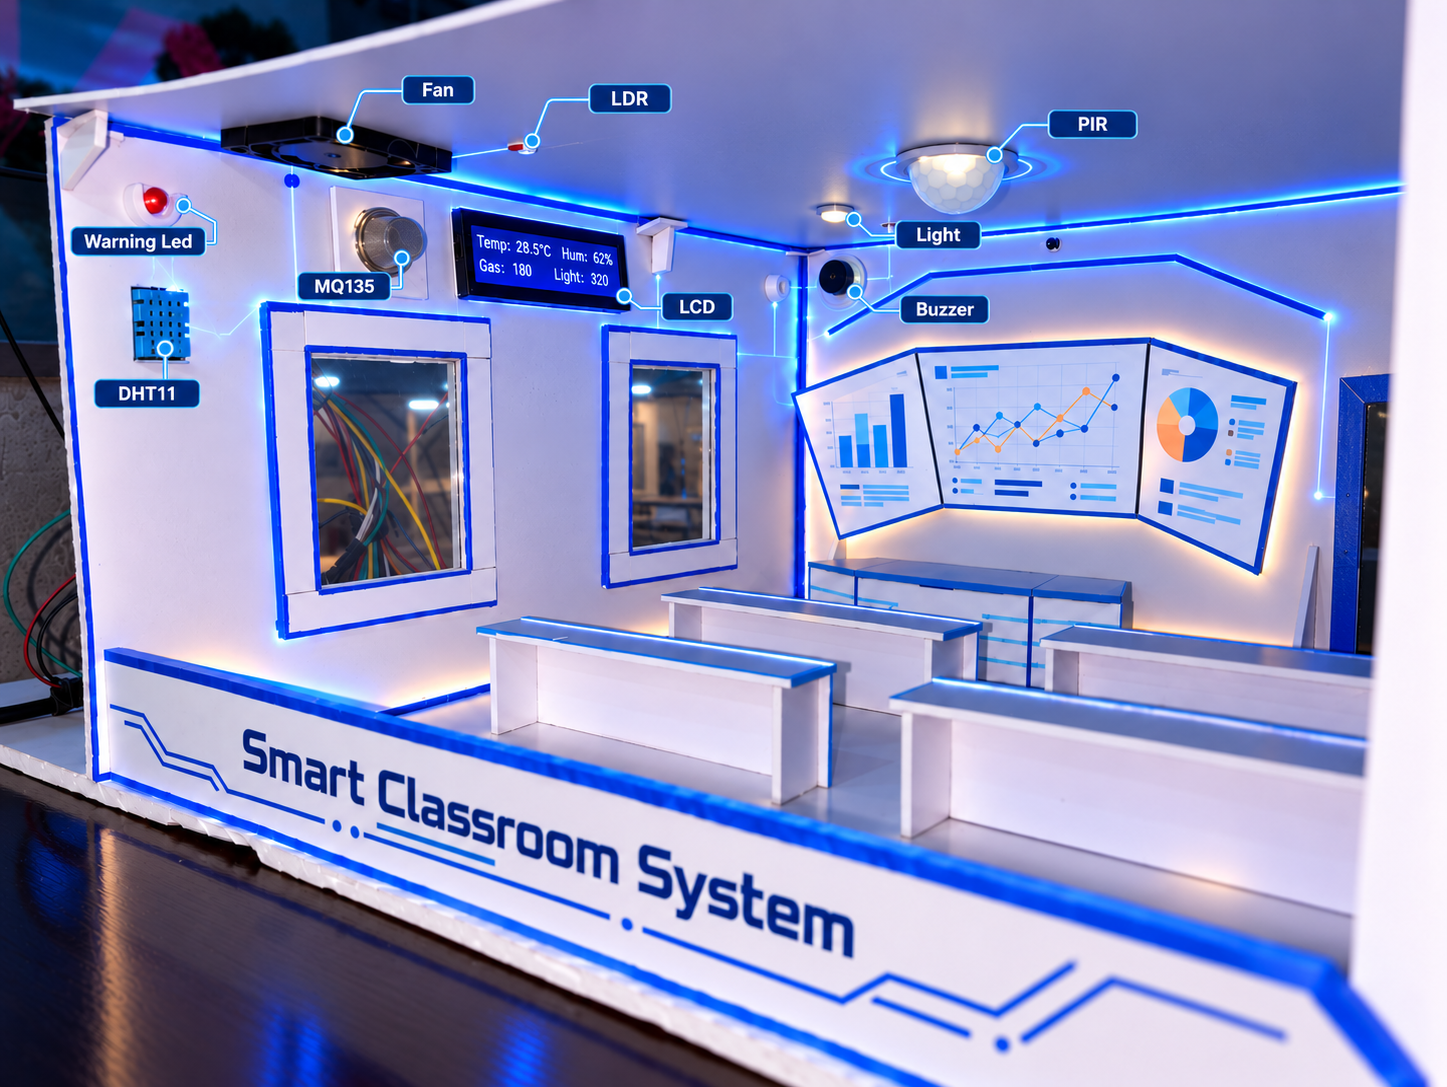
\includegraphics[width=\textwidth, height=4.2cm]{Smart Classroom System Diorama.png}
        \caption{Mô hình Diorama phòng học thực tế}
        \label{fig:sub_diorama}
    \end{subfigure}
    \hfill
    \begin{subfigure}[b]{0.48\textwidth}
        \centering
        \fbox{\parbox[c][4.2cm][c]{0.95\textwidth}{\centering \textbf{[Ảnh Bo mạch ESP8266 \& Cảm biến]}\\ \small File đính kèm: \texttt{hardware\_board.png}}}
        \caption{Bo mạch điều khiển NodeMCU V3 \& Cụm cảm biến}
        \label{fig:sub_board}
    \end{subfigure}
    
    \vskip 0.4cm
    
    \begin{subfigure}[b]{0.48\textwidth}
        \centering
        \fbox{\parbox[c][4.2cm][c]{0.95\textwidth}{\centering \textbf{[Ảnh Giao diện Web Dashboard]}\\ \small File đính kèm: \texttt{web\_dashboard.png}}}
        \caption{Giao diện điều khiển Web Server Port 80}
        \label{fig:sub_web}
    \end{subfigure}
    \hfill
    \begin{subfigure}[b]{0.48\textwidth}
        \centering
        \fbox{\parbox[c][4.2cm][c]{0.95\textwidth}{\centering \textbf{[Ảnh Email Cảnh báo HTML]}\\ \small File đính kèm: \texttt{email\_alert.png}}}
        \caption{Email HTML cảnh báo sự cố khẩn cấp}
        \label{fig:sub_email}
    \end{subfigure}
    \caption{Tập hợp hình ảnh phần cứng thực tế và giao diện ứng dụng của hệ thống}
    \label{fig:prototype_gallery}
\end{figure}

% ------------------------------------------------------------------------------
% S11: TRÌNH DIỄN DEMO, TEST CASES & MÃ QR CODE
% ------------------------------------------------------------------------------
\section{Kịch Bản Kiểm Thử (Test Cases) \& Mã QR Video Demo (S11)}

\subsection{Bảng Tổng Hợp 4 Kịch Bản Kiểm Thử Trọng Yếu}
Nhóm nghiên cứu đã thực hiện 4 kịch bản kiểm thử trực tiếp trước Hội đồng để xác thực năng lực phản xạ của hệ thống (Bảng~\ref{tab:test_cases}).

\begin{table}[htbp]
    \centering
    \caption{Kết quả thực nghiệm 4 kịch bản kiểm thử (Test Cases Verification)}
    \label{tab:test_cases}
    \begin{tabular}{@{}lp{4.2cm}p{5.5cm}c@{}}
        \toprule
        \textbf{Kịch Bản} & \textbf{Thao Tác Thực Hiện} & \textbf{Phản Ứng Của Hệ Thống} & \textbf{Kết Quả} \\
        \midrule
        \textbf{TC1: Quá nhiệt} & Dùng máy sấy gia nhiệt vào DHT11 lên $T \ge 35.0^\circ\text{C}$. & Quạt tự bật, LED đỏ chớp, Web báo động, Gửi Email. \textbf{Tuyệt đối không hú còi} để tránh ảnh hưởng lớp học kế bên. & \textbf{PASSED} \\
        \addlinespace
        \textbf{TC2: Rò rỉ Gas} & Xả bật lửa gas vào cảm biến MQ135 ($\text{ADC} \ge 500$). & Quạt bật tối đa thông gió, gửi Email khẩn cấp, \textbf{Còi hú ầm ĩ liên tục} vì sự cố đe dọa sinh mạng. & \textbf{PASSED} \\
        \addlinespace
        \textbf{TC3: Tiết kiệm điện} & Che tối LDR và vẫy tay qua cảm biến PIR. & Đèn học LED tự bật. Khi ngừng chuyển động, \textbf{đèn sáng thêm 15 giây} rồi mới tắt, chống tắt đột ngột khi ngồi ghi bài. & \textbf{PASSED} \\
        \addlinespace
        \textbf{TC4: Safety Override} & Bấm nút TẮT quạt trên Web, sau đó xả khí gas vào MQ135. & Edge Logic tự động \textbf{ghi đè quyền điều khiển thủ công}, cưỡng bức bật quạt thông gió để đảm bảo an toàn. & \textbf{PASSED} \\
        \bottomrule
    \end{tabular}
\end{table}

\subsection{Mã QR Code Truy Cập Video Demo \& Kho Mã Nguồn}
Quét mã QR dưới đây bằng camera điện thoại để truy cập trực tiếp vào Video trình diễn thực tế và kho mã nguồn hoàn chỉnh của dự án (Hình~\ref{fig:qr_codes}).

\begin{figure}[htbp]
    \centering
    \begin{minipage}{0.45\textwidth}
        \centering
        % Mã QR tự động sinh bằng gói qrcode
        \qrcode[height=3.8cm]{https://www.youtube.com/watch?v=dQw4w9WgXcQ}\\[0.3cm]
        \textbf{Video Demo Trình Diễn (YouTube)}\\
        \small\url{https://www.youtube.com/watch?v=dQw4w9WgXcQ}
    \end{minipage}
    \hfill
    \begin{minipage}{0.45\textwidth}
        \centering
        % Mã QR tự động sinh bằng gói qrcode
        \qrcode[height=3.8cm]{https://github.com/smartclassroom-iot/esp8266-core}\\[0.3cm]
        \textbf{Mã Nguồn Toàn Bộ Dự Án (GitHub)}\\
        \small\url{https://github.com/smartclassroom-iot/esp8266-core}
    \end{minipage}
    \caption{Mã QR tương tác truy cập Video YouTube và GitHub Repository}
    \label{fig:qr_codes}
\end{figure}

\newpage
% ------------------------------------------------------------------------------
% S12: TỔNG KẾT KẾT QUẢ ĐẠT ĐƯỢC
% ------------------------------------------------------------------------------
\section{Tổng Kết Kết Quả Đạt Được (S12)}

Dự án đã hiện thực hóa thành công mô hình phòng học thông minh với những thành tựu nổi bật:
\begin{enumerate}
    \item \textbf{Kiến trúc Non-blocking thuần túy:} Toàn bộ mã nguồn loại bỏ triệt để các hàm ngắt thực thi \texttt{delay()}, ứng dụng bộ điều phối thời gian \texttt{millis()} độc lập cho từng tác vụ (đọc cảm biến $2\,\text{s}$, chớp đèn báo động $300\,\text{ms}$, đổi màn hình LCD $2\,\text{s}$). Điều này đảm bảo Web Server phản hồi trong thời gian thực $< 50\,\text{ms}$.
    \item \textbf{Phản xạ ngắt phần cứng tức thời:} Ứng dụng ngắt ngoài phần cứng (\texttt{Hardware ISR}) trên chân D5 cho cảm biến PIR giúp ghi nhận sự hiện diện của học sinh ngay lập tức mà không phụ thuộc vào chu kỳ quét lặp.
    \item \textbf{Logic cảnh báo thông minh \& Chống bão thư rác:} Cơ chế cờ nhớ trạng thái leo thang (\textit{Escalation Flags}) kết hợp bộ đếm Cooldown $300.000\,\text{ms}$ ($5\,\text{phút}$) giúp hộp thư người quản lý không bị tràn dữ liệu khi xảy ra sự cố kéo dài.
    \item \textbf{Cơ chế dự phòng an toàn đa tầng (Fail-safe):} Tính năng AP Fallback tự phát Hotspot \texttt{192.168.4.1} khi rớt mạng trường đảm bảo hệ thống vận hành bền bỉ $24/7$.
\end{enumerate}

% ------------------------------------------------------------------------------
% S13: ĐỊNH HƯỚNG PHÁT TRIỂN TƯƠNG LAI
% ------------------------------------------------------------------------------
\section{Định Hướng Nghiên Cứu \& Phát Triển Tương Lai (S13)}

Để mở rộng hệ thống phục vụ quy mô toàn trường đại học, nhóm đề xuất ba hướng nâng cấp chiến lược:
\begin{itemize}
    \item \textbf{Chuyển dịch sang Giao thức MQTT \& Nền tảng IoT Cloud:} Triển khai Broker MQTT (HiveMQ hoặc AWS IoT Core) với mô hình Xuất bản / Đăng ký (\textit{Pub/Sub}) siêu nhẹ. Điều này cho phép một máy chủ trung tâm quản trị đồng thời hàng trăm phòng học xuyên suốt mạng diện rộng Internet.
    \item \textbf{Tích hợp Thị giác máy tính tại biên (Camera AI ESP32-CAM):} Nâng cấp module ESP32-CAM chạy các mô hình học máy TinyML nhằm tự động điểm danh sinh viên qua nhận diện khuôn mặt và đếm chính xác số người trong phòng học để điều chỉnh công suất quạt/điều hòa theo mật độ thực tế.
    \item \textbf{Đo lường năng lượng chuyên sâu với PZEM-004T:} Tích hợp biến dòng PZEM-004T đo trực tiếp điện áp ($V$), dòng điện ($A$), công suất tác dụng ($W$) và điện năng tiêu thụ ($kWh$). Hệ thống có thể tính toán chi phí tiền điện tức thì và cảnh báo nguy cơ quá tải đường dây điện.
\end{itemize}

% ------------------------------------------------------------------------------
% S14: LỜI CẢM ƠN & PHIÊN HỎI ĐÁP Q&A
% ------------------------------------------------------------------------------
\section{Lời Cảm Ơn \& Phiên Thảo Luận (Q\&A Session) (S14)}

Nhóm nghiên cứu xin trân trọng gửi lời cảm ơn sâu sắc tới các Thầy Cô trong Bộ môn Kỹ thuật Máy tính \& IoT, Khoa Công nghệ Thông tin đã tận tình định hướng, hướng dẫn phương pháp luận và tạo điều kiện về trang thiết bị thí nghiệm trong suốt quá trình hoàn thiện đồ án.

\vspace{0.8cm}
\begin{center}
    \begin{tcolorbox}[colback=boxBgCyan, colframe=iotCyan, width=0.88\textwidth, arc=8pt, boxrule=1.5pt, halign=center]
        \vspace{0.3cm}
        {\Large \textbf{\color{iotDark} PHIÊN HỎI \& ĐÁP (Q\&A SESSION)}}\\[0.3cm]
        {\large \textit{Kính mời Quý Thầy Cô trong Hội đồng Đánh giá đặt câu hỏi\\và đóng góp ý kiến phản biện để đề tài được hoàn thiện hơn!}}\\[0.3cm]
        \vspace{0.2cm}
    \end{tcolorbox}
\end{center}

\end{document}

